\section{Introduction}
\label{Introduction}
The atmospheric radiation environment is highly complex and is comprised mostly of a mix of primary and secondary particles originating from Galactic Cosmic Rays (GCRs). Primary GCRs interact with atoms and molecules in the Earth's upper atmosphere and produce cascades of secondary particles that increase in intensity until reaching a maximum between 16km and 18km, known as the Regener-Pfotzer Maximum. After reaching peak ionization rates, the flux of secondary and primary particles then decreases steadily until reaching a minimum near the earths surface. The increase in ionizing radiation with altitude has implications to passengers and crew aboard high flying aircraft and astronauts in low earth orbit (LEO), who will absorb a much higher biological dose than they would at the earths surface. According to research from the Federal Aviation Administration (FAA) Civil Aerospace Medical Institute, passengers and crew onboard a flight from London to Los Angeles will be exposed to an average effective dose of \SI{61.6}{\micro\sievert}\cite{faa} and measurements taken aboard the International Space Station (ISS) shows that ISS crew members can be exposed to dose rates on the order of \SI{200}{\micro\sievert} per day. Exposure to high levels of ionizing radiation increases the risk of cancer and may be linked to other health risks such as increased rate of birth defects and miscarriages\cite{flightatt}. 
%Paper for miscarriages and birth defects
%Another possible source: https://www.ncbi.nlm.nih.gov/pmc/articles/PMC4510952/ and further confirmed by: https://www.cdc.gov/niosh/topics/aircrew/reproductivehealth.html
%s. "For flight attendants, a NIOSH study found that exposure to 0.1 mGy (0.36 mSv) or more of cosmic radiation in the first trimester may be linked to increased risk of miscarriage"
Additionally, data from the CRaTER cosmic ray telescope aboard NASA’s Lunar Reconnaissance Orbiter has shown that dose rate from cosmic rays on the moons surface has been increasing over the last 50 years and is predicted to reach a historical maximum in 2020 at the lowest point of the ongoing solar minimum\cite{crater}. The health risks associated with exposure to radiation in the atmosphere and in space combined with the increase in cosmic ray intensity seems to increasingly point towards the necessity of the development of a relatively low cost device for monitoring the radiation environment in real-time.

The MiniPIX is a portable radiation camera developed by Advacam that utilizes a 256x256 pixel silicon TimePIX Application Specific Integrated Circuit (ASIC) and a USB readout interface. The device can be operated under one of three modes: time-of-arrival (TOA), time-over-threshold (TOT), or single particle counting. The MiniPIX is capable of individual particle differentiation and, when operating in TOT mode can be used to measure dosimetric endpoints such as absorbed dose and dose equivalent. Similar devices to the MiniPIX utilizing a TimePIX ASIC have been evaluated on high altitude balloon flights by Urbar et.al\cite{bexus} and are currently deployed on the ISS for performing real-time space radiation monitoring\cite{timepixiss}. However, the usage of the MiniPIX in combination with a low cost single board computer as a portable radiation monitoring device has yet to be fully explored. The SORA flights in 2017 and 2018 served as a test bed for such a system.

%Space radiation and galactic cosmic rays (GCRs) pose real health risks to astronauts and pilots in any field.  Radiation exposure in Low Earth Orbit and the atmosphere must be monitored to ensure they do not exceed the occupational dose limits.  The ability to measure real-time exposure is arguably a crucial tool that can help mitigate risks.  Studying radiation types and dose levels near the nebulous border between space and Earth's atmosphere, and within the various zones of the atmosphere, facilitates preparation for current and future space missions; and aviation in general.  

%To monitor the radiation in the upper atmosphere and beyond, a USB TimePIX device could be effectively used as a low cost dosimeter.  TimePIX detectors have many applications in the realm of particle physics, specially with their small physical and power consumption footprint. Overall, TimePIX devices could be setup to create a network of devices to better understand the Earth space radiation environment and observe space weather.
%
%Numerous balloon flights have included the use of TimePIX devices for the purposes of particle imaging and radiation dosimetry in unusual and unfamiliar environments, such as the stratosphere \cite{bexus}. 
%
%The International Space Station (ISS) uses TimePIX devices to evaluate the astronauts' exposure to ionizing radiation fields \cite{timepix}.
% below is an actual space

%The TimePIX device used in this flight was a MiniPIX, which is a silicon-based hybrid pixel detector built by ADVACAM \cite{advacam}. 
%
%The sensor surface offers a resolution of 256x256 pixels.
%The device can be operated under one of three modes: time-of-arrival (TOA) or time-over-threshold (TOT), or single particle counting. When a charged particle interacts with the silicon chip, ionization currents are created which are detected and measured by the device.

\begin{figure}[H]
    \centering
    %%%%%%%%%%%%%%%change to width=0.35\textwidth for print
    %width=/textwidth for review
    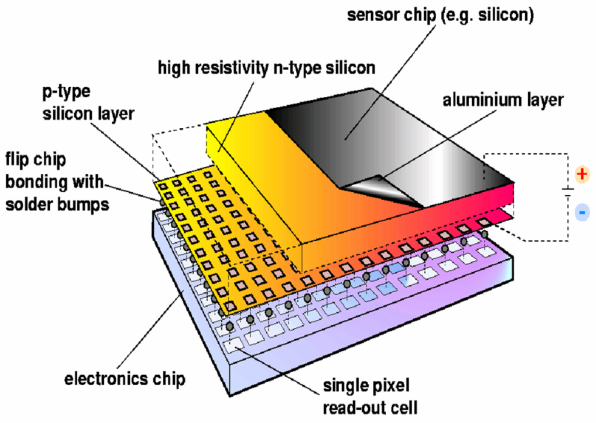
\includegraphics[width=\textwidth]{minipix_silicon.pdf}
    \caption{MiniPIX silicon concept design}
    \label{fig:minipix_silicon}
\end{figure}

During the High Altitude Student Platform (HASP) 2017 and 2018 flights \cite{hasp}, the SORA payload carried a MiniPIX silicon-chip hybrid pixel detector interfaced with a Raspberry Pi Single Board Computer to test the feasibility of such a system for real-time measurements of absorbed dose from cosmic radiation. Data from the MiniPIX was analyzed in real time and counts and absorbed dose were downlinked in real time through the HASP downlink interface. The HASP 2017 flight launched from Fort Sumner, New Mexico on September 4th, 2017 at 14:04 UTC and ascended to a float altitude of approximately $\SI{31.5}{\kilo\meter}$ at 16:22 UTC; which was maintained for approximately \SI{10.5}{\hour}. On September 4th, 2018 at 14:03 UTC the HASP 2018 mission also launched from Fort Sumner, Mew Mexico.  The 2018 payload reached a stable float altitude of $\SI{37.2}{\kilo\meter}$ at 16:30 UTC and the total float duration was approximately \SI{9.0}{\hour}. The first payload drifted west for a total ground distance of \SI{580}{\kilo\meter} and was recovered just north of the Apache-Sitgreaves National Forest in Arizona. The 2018 payload terminated its flight and landed approximately \SI{96.6}{\kilo\meter} southwest of Mt Graham, Arizona after traveling a total distance of \SI{550}{\kilo\meter}.
%
%
%
%%%%%%%%%MERGE Background %%%%%%%%%%%%
%
%
%
% I suggest we discuss briefly Timepix detectors use on the ISS and other places for space radiation dosimetry and particle identification. We can also talk a bit about our motivations of studying cosmic rays on commercial airline flights.
%
% Find model to fit our data
%
% Mention motivation for study, such as GCR's, seeing the Regener-Pfotzer Maximum, space flight and radiation importance, commercial air flights.  LOW COST RAPSBERRY PI SYSTEM.
%
%\section{Background}
%\label{Background}
%%% GCR's and Regener-Pfotzer Maxiumum, space flight ----- Work in Progress

%Space radiation and galactic cosmic rays (GCRs) pose real health risks to astronauts and pilots in any field.  Radiation exposure in Low Earth Orbit and the atmosphere must be monitored to ensure they do not exceed the occupational dose limits.  The ability to measure real-time exposure is arguably a crucial tool that can help mitigate risks.  Studying radiation types and dose levels near the nebulous border between space and Earth's atmosphere, and within the various zones of the atmosphere, facilitates preparation for current and future space missions; and aviation in general.  
%
%To monitor the radiation in the upper atmosphere and beyond, a USB TimePIX device could be effectively used as a low cost dosimeter.  TimePIX detectors have many applications in the realm of particle physics, specially with their small physical and power consumption footprint. Overall, TimePIX devices could be setup to create a network of devices to better understand the Earth space radiation environment and observe space weather.
%%
%%
%%%%   Lets tie this together, actual space below
%%
%%
%Numerous balloon flights have included the use of TimePIX devices for the purposes of particle imaging and radiation dosimetry in unusual and unfamiliar environments, such as the stratosphere \cite{bexus}. 
%%
%The International Space Station (ISS) uses TimePIX devices to evaluate the astronauts' exposure to ionizing radiation fields \cite{timepix}.
%% below is an actual space
%
%The TimePIX device used in this flight was a MiniPIX, which is a silicon-based hybrid pixel detector built by ADVACAM \cite{advacam}. 
%%
%The sensor surface offers a resolution of 256x256 pixels.
%%
%The device can be operated under one of three modes: time-of-arrival (TOA) or time-over-threshold (TOT), or single particle counting. 
%%
%%When a particle ionizes with the silicon chip, the deposited charge is depleted by a bias voltage in a process known as Carrier generation and recombination. \textbf{<<Verify the previous statement>>}
%%I think we can simplify this statement into this, since we don't have to go too deep into the background.  Just the basics works.
%When a charged particle interacts with the silicon chip, ionization currents are created which are detected and measured by the device.
%
%\begin{figure}[h]
%    \centering
%    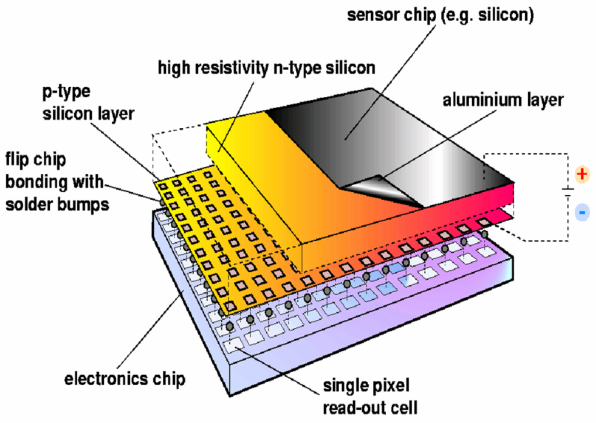
\includegraphics[width=0.35\textwidth]{minipix_silicon.pdf}
%    \caption{MiniPIX silicon concept design}
%    \label{fig:minipix_silicon}
%\end{figure}
%
%figure name: minipix_silicon.pdf
%

%This was copied over to the "Experiment Design Section"
%For the SORA flights, the MiniPIX was coupled with a low cost open ARM based computer.  Both flights utilized a Raspberry Pi 3 to communicate and handle all operations with the MiniPIX.  This system allowed for remote operation and on-board analyzation of all data.  The SORA flights tested the feasibility of these low-cost systems to fly further space missions.  

